In this section, we provide a security analysis of the effectiveness and robustness of \scheme{}.
We define security in this context as follows: \scheme{} succeeds if an attacker cannot distinguish, with non-negligible advantage, between a Security Sensitive access to a near-tile LLC bank and one to a far-tile LLC bank based on observed latency.

\begin{figure*}[t]
    \centering
    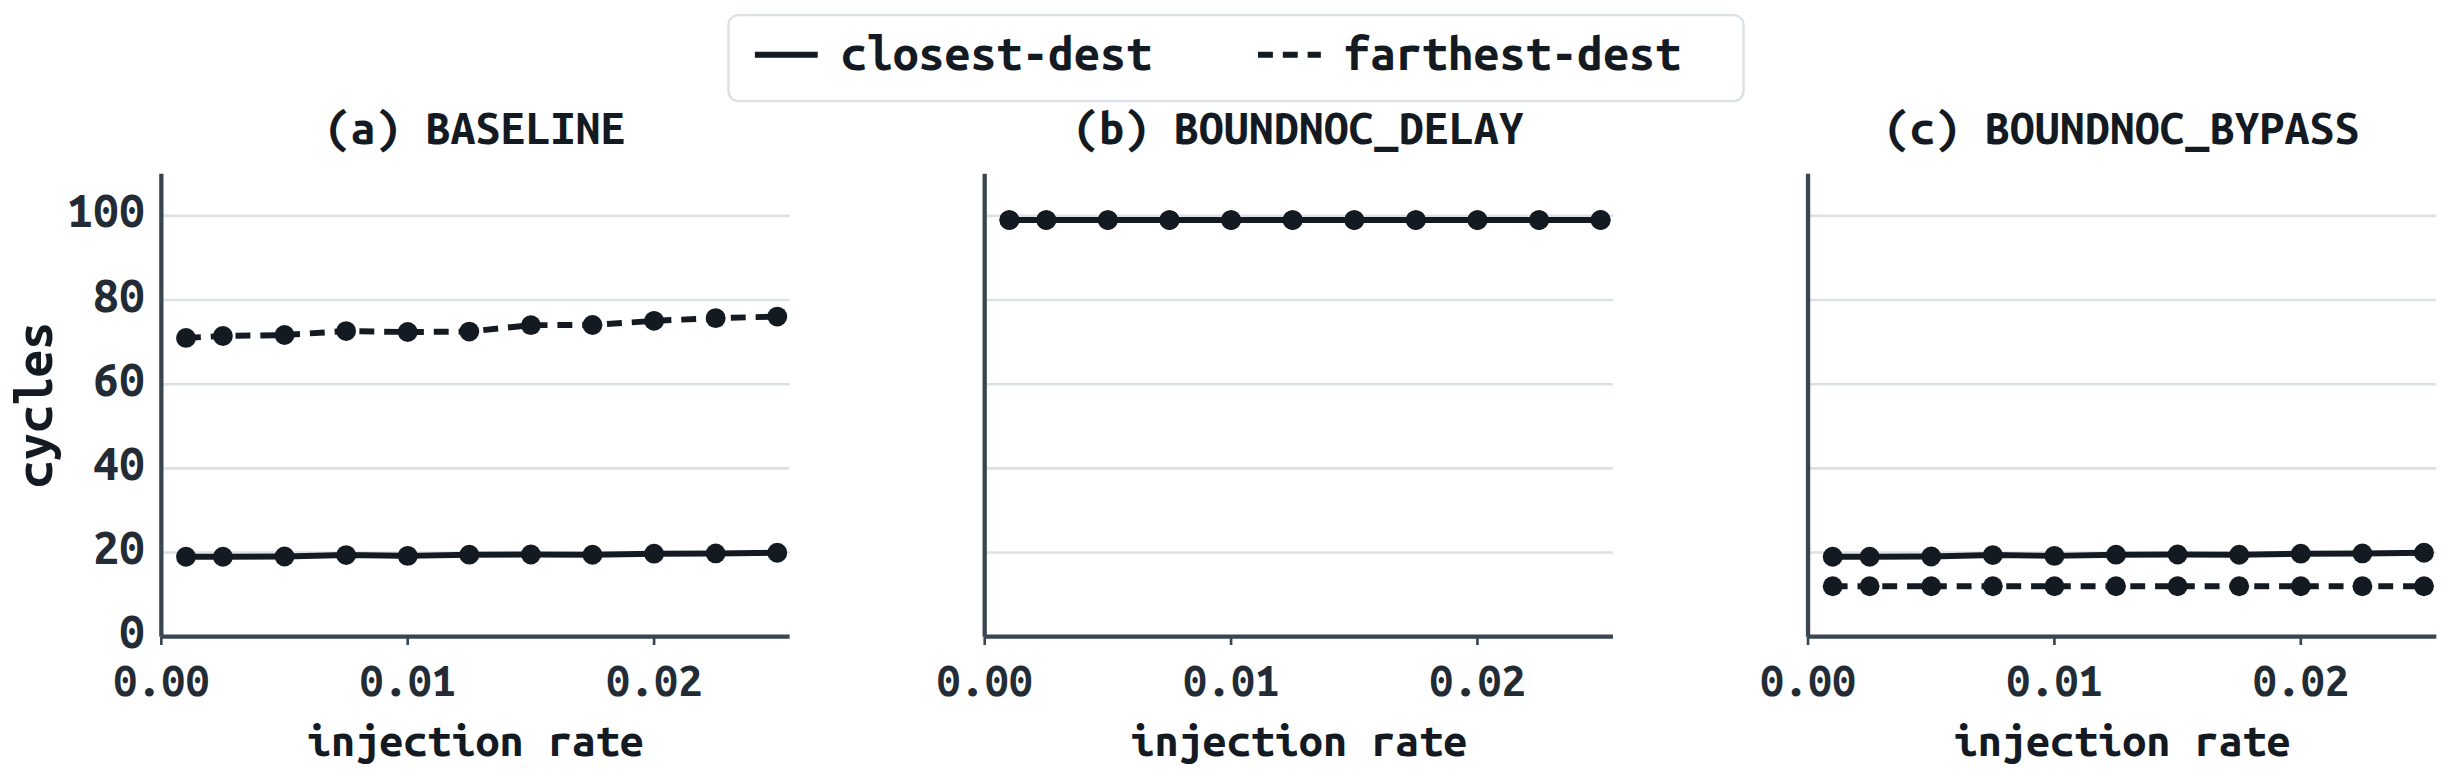
\includegraphics[width=0.85\linewidth]{figs_new/boundnoc_roundtrip_latency_syn.png}
    %{figs/attack-packet.pdf}
    \caption{Impact of different policies on Secure Load round-trip latency for a synthetic workload.
    (a)~\basescheme{}: near-tile and far-tile latencies are clearly separable.
    (b)~\jscheme{}: latencies are indistinguishable but elevated.
    (c)~\bscheme{}: latencies are indistinguishable with near-optimal absolute latency.}
    \label{fig:impact-on-latency-syn}
\end{figure*}

\subsection{\jscheme} \label{sec-security-jscheme}
In \jscheme{}, the timing difference between a nearby LLC access and a faraway LLC access is mitigated by adding delays to sensitive LLC accesses at the source NI.
The LLC access latency in \cpumodel{} consists of two parts: the latency to the CHA, and the latency to the LLC slice storing the cache line.
Since the latter depends on which core brought the cache line into the LLC and is unlikely to exhibit observable patterns to the attacker, our main mitigation target is the latency to the CHA, which is determined by the physical address via a hash function.
To eliminate observable patterns, \jscheme{} makes every LLC-hit access a constant-time operation regardless of distance.

We evaluate \jscheme{} by comparing the round-trip latency of far-tile and near-tile cache line accesses at various injection rates.
As shown in Figure~\ref{fig:impact-on-latency-syn}(b), the round-trip latency of a Security Sensitive load with \jscheme{} shows no difference based on distance at injection rates from 0.000 to 0.357.
Note that \jscheme{} provides this guarantee only until the NoC becomes saturated.
Under saturation, LLC latency far exceeds the average and becomes non-deterministic, making it impossible for an attacker to extract reliable distance-based patterns.
We observe that the network saturates at injection rate 0.357, where the round-trip latency does not exceed $T_{worst}=100$ cycles.
Therefore, 100 cycles is a safe delay threshold for \jscheme{}.

\subsection{\bscheme} \label{sec-security-bscheme}
In \bscheme{}, the timing difference is mitigated by enforcing a lower target latency $T_{low}$, defined in Equation~\ref{eq:tlow}, rather than $T_{worst}$.
$T_{low}$ combines the worst-case latency from the source to the CHA, the worst-case latency from the CHA to the destination, and the minimum achievable latency from the destination back to the source using bypass.
For a Security Sensitive packet $p$, there are three scenarios:

\begin{compactenum}[(1)]
    \item The expected round-trip latency without bypass (${EL}_{p}$) is at most $T_{low}$.
    No bypass is needed; \bscheme{} delivers the packet after adding delay to match $T_{low}$.

    \item ${EL}_{p}$ exceeds $T_{low}$, but after applying bypass the actual round-trip latency falls below $T_{low}$.
    This is the common case: \bscheme{} uses router bypass to expedite delivery of $p$ and then adds delay to match $T_{low}$.

    \item ${EL}_{p}$ exceeds $T_{low}$ and the round-trip latency remains above $T_{low}$ even after bypass, which occurs only under network saturation.
    In this case, the observed latency is dominated by non-deterministic congestion rather than distance-dependent LLC access patterns, so an attacker cannot reliably distinguish near-tile from far-tile accesses.
\end{compactenum}

Figure~\ref{fig:impact-on-latency-syn}(c) shows the round-trip latency of a Security Sensitive load with \bscheme{}, confirming no observable difference based on distance at injection rates 0.000 to 0.357.

\subsection{Defense Against Congestion-Based Attacks}
\scheme{} defends against congestion-based attacks by ensuring all Security Sensitive packets are delivered within $T_{low}$, regardless of network congestion.
Since the observed latency is always $T_{low}$, an attacker cannot infer whether the traffic by the victim created congestion on any particular network path.

\subsection{Resistance to Bypass Contention Channel}
Although an attacker could in principle attempt to use the bypass mechanism as a contention channel, \bscheme{} provides no exploitable signal through this channel.
Bypass is applied deterministically based on expected latency rather than on any secret-dependent condition, so bypass usage reveals nothing about the memory access pattern of the victim.
Furthermore, \bscheme{} applies bypass indiscriminately whenever $EL_p > T_{low}$, so the attacker cannot infer contention based on whether bypass is used.
In our experiments (Section~\ref{sec:eval}), the maximum wait time to acquire the bypass path is 2 cycles under non-saturated network conditions, keeping the latency bound tight and predictable.
